
%----------------------------------------------------------------------------------------------------------------------------------------

% définit le type de document et ses options
\documentclass[a4paper,10pt]{article}

% des paquetages indispensables, qui ajoutent des fonctionnalites
\usepackage[utf8]{inputenc}
\usepackage{graphicx}
\usepackage{lscape}
\usepackage{url}
\usepackage{xspace}
\usepackage[francais]{babel}
%\usepackage{fullpage}

\pagestyle{plain}


%----------------------------------------------------------------------------------------------------------------------------------------


% le debut du contenu
\begin{document}


%----------------------------------------------------------------------------------------------------------------------------------------

%%%%%%%%%%%%%%%%%%%%%%%%%%%%%%%%%%%%%%%%%%%%%%%%%
%%Page d'accueil
\begin{center}
	%%
	\hspace{3cm}
	
\includegraphics[scale=0.8]{logo.ps}

	%%
	\vspace{1cm}
	{\large Projet de spécialité 2010}\\
	{\Large Conception d'un modèle de feu 3D temps réel}\\
	{\large Organisation du projet}\\
	\vspace{1cm}


	\includegraphics[scale=0.3]{feu.ps}\\
	\vspace{2cm}
	%%
	Etudiants impliqués :\\
	Benjamin Aupetit - IRVM - benjamin.aupetit@ensimag.imag.fr\\
	Julien Champeau - IRVM - julien.champeau@ensimag.imag.fr\\
	Arnaud Emilien - IRVM - arnaud.emilien@ensimag.imag.fr\\
	~\\
	Encadrants :\\
	Marie-Paule Cani  -  Marie-Paule.Cani@inrialpes.fr \\
	Aurélie Catel - aurelie.catel@grenoble-inp.fr
	~ \\
	\vspace{3mm}
	Ensimag 2010\\

\end{center}

\newpage

\tableofcontents

\newpage









%----------------------------------------------------------------------------------------------------------------------------------------
%%%%%%%%%%%%%%%%%
\section{Constitution de l'équipe}
%%%%%%%%%%%%%%%%%

\subsection{Choix du sujet}

Dans notre cursus IRVM nous avons assisté au cours "Graphique 3D" que nous avons particulièrement aprécié. Cette discipline est particulièrement indispensable à l'industrie du jeux vidéo, du film d'animation, ... \\
L'étude d'un phénomène réel, la conception de son modèle et la réalisation d'une application 3D temps réel est un procédé qui nous interesse particulièrement. Actuellement, aucun des sujets présentés ne propose cette démarche.\\
Cette discipline est d'autant plus importante pour nous que nous souhaitons en faire notre métier. Le projet de spécialité est une occasion unique de travailler à temps plein sur une problématique passionante, qui nous permettrait d'aquérir un savoir et des compétences importantes. Ce serait une réelle valeur ajouté dans notre bagage scolaire.\\
~\\
La modélisation du feu est un domaine interessant car il fait le lien entre de nombreux principes physiques, de nombreux modèles mathématiques, de nombreuses méthodes de calcul et de rendu. De plus la contrainte temps réel permet de ne garder que les éléments importants pour la visualisation, en simplifiant les modèles.

\subsection{Choix des membres}
\subsubsection{Arnaud}
\subsubsection{Benjamin}
\subsubsection{Julien}


\subsection{Forces et faiblesses de l'équipe}


%----------------------------------------------------------------------------------------------------------------------------------------
%%%%%%%%%%%%%%%%%
\section{Charte de travail}
La charte de travail a été établie dans le but de réaliser le plus de
points de notre sujet dans les délais impartis.  \\

Nous avons réparti le travail de façon homogène entre les membres de
l'équipe.  Nous nous sommes mis d'accord sur notre façon de travailler
: chacun d'entre nous utilise son propre ordinateur, nous utilisons un
gestionnaire de version ( «git» ) et nous nous sommes mis d'accord sur
une convention de codage et de commentaire. \\

Avant, et après, chaque rencontre avec notre tutrice. Avant pour
établir l'ordre du jour, discuter des point à discuter et/ou mettre en
avant. Et après pour en faire un bilan sur le déroulement de la
réunion et en déduire des éventuels changements d'orientation. \\

Pour les horaires de travail nouas avons choisis de travailler tous
les jours sauf le dimanche, de 9h à 17h et nous avons décidé de faire
un mini bilan sur ce que nous avons fait à la fin de chaque journée.\\

Les rôles ont été définis ainsi, en prenant en compte les points forts
de chacun :\\

\begin{itemize}

\item \textbf{Arnaud}
\begin{itemize}
\item bonne connaissance d'OpenGL.
\end{itemize}
\quad \\

\item \textbf{Benjamin}
\begin{itemize}
\item bon niveau en C++
\item familier avec l'analyse de problèmes et la modélisation en UML
\end{itemize}
\quad \\

\item \textbf{Julien}
\begin{itemize}
\item interêt pour l'informatique graphique
\item apprecie la modélisation de phénomènes physique
\end{itemize}
\quad \\

\end{itemize}
%%%%%%%%%%%%%%%%%

%----------------------------------------------------------------------------------------------------------------------------------------
%%%%%%%%%%%%%%%%%
\section{Planning prévisionnel}
%%%%%%%%%%%%%%%%%

	\includegraphics[scale=0.8]{../Planning/GANTT.ps}
	
	\includegraphics[scale=0.8]{../Planning/Planning.ps}


%----------------------------------------------------------------------------------------------------------------------------------------
%%%%%%%%%%%%%%%%%
\section{Répartition du travail}
%%%%%%%%%%%%%%%%%


%----------------------------------------------------------------------------------------------------------------------------------------
%%%%%%%%%%%%%%%%%
\section{Déroulement du projet}
%%%%%%%%%%%%%%%%%

%----------------------------------------------------------------------------------------------------------------------------------------
%%%%%%%%%%%%%%%%%
\section{Compte rendu des réunions}
%%%%%%%%%%%%%%%%%

%%%%%%%%%%%%%%%%%
\subsection{Suivis du  20 mai 2010}
%%%%%%%%%%%%%%%%%

\subsubsection{Présents}
\textbf{Tuteur} : Marie Paule Cani \\
\textbf{Élèves} : Benjamin, Julien, Arnaud \\

\subsubsection{Sujets abordés}
\textbf{Définition du but et de l'échelle du projet} :  \\
se concentrer sur la propagation et la destruction des objets.\\

\textbf{Pistes à regarder} : \\
Jos Stam a fait de nombreux travaux à ce sujet, il faut regarder sur son site web de toronto. Par exemple : burning cross. Il a travaillé sur la représentation et  les modèles de feu temps réel.\\
Mathieu Desbrun à fait "Voxels On fire" et "Meshes On Fire", deux travaux sur la propagation temps réel du feu sur un objet.\\
Représentation du feu par voxels.\\

\textbf{Conseil sur la démarche} : \\
Reflechir beaucoup au BUT,
identifier les phénomènes importants,
lire beaucoup,
faire des résumés régulièrement.\\

\subsubsection{Prochain rendez vous}
Lundi 31, à 10h à l'INRIA.\\
Nous devrons y présenter le modèle de feu et de fumée.



%%%%%%%%%%%%%%%%%
\subsection{Suivis du  31 mai 2010}
%%%%%%%%%%%%%%%%%
\subsubsection{Présents}
\textbf{Tuteur} : Marie Paule Cani\\
\textbf{Élèves} : Benjamin, Julien, Arnaud \\
\textbf{Et aussi : un chercheur de l'INRIA} : Cyril Crassin \\

\subsubsection{Sujets abordés}
\textbf{Présentation de l'avancement du projet} :  \\
    Nous avons présenté à notre tutrice le modèle de fluide que nous avons implémenté en CPU.
    Nous avons expliqué son fonctionnement, comment nous étions arrivés à ces résultats, 
    quels étaient les articles qui nous avaient le plus aidé.\\
    Notre tutrice semblait satisfaite du travail effectué.\\
    
\textbf{Explication de l'implémentation, discussion à propos des modifications/améliorations à apporter} :  \\
    Nous discuté à propos des améliorations du rendu, notamment de l'ajout d'un bruit de perlin à la texture.\\
    Nous avons aussi parlé de la fumée qui doit être générée d'un autre façon.\\
    Nous avons de même parlé de la flamme qui doit perdre progressivement de la matière ( diminution du combustible présent )\\
    
\textbf{Discussions à propos du travail futur} :  \\
    Nous avons parlé de plusieurs manières d'ajouter des objets au modèle de fluide, 
    pour dégager le modèle le plus adéquat. En effet nous avions trouvé beaucoup de modèles 
    possibles mais avions du mal à en choisir un. Avec les nouvelles pistes de 
    réflexions et avec les conseils de notre tutrice nous allons pouvoir effectuer
    ce choix plus facilement.\\
    
\textbf{Résolution des problèmes liés à la version GPU} :  \\
    Dans le but de nous aider à comprendre les problèmes de notre version GPU, 
    notre tutrice nous à fait rencontrer Cyril Crassin, un chercheur de l'INRIA qui
    a beaucoup travaillé sur le GPU. Il a su répondre parfaitement à nos questions,
    ce court dialogue a été extremement profitable. \\

\subsubsection{Prochain rendez vous}
Le prochain rendez-vous sera fixé dans la semaine par mail. Il s'agira sans doute de ventredi 4 Juin.\\
Nous devrons présenter la version corrigée de notre modèle de fluide et un début d'implémentation de propagation
sur objets.\\

\subsection{Suivi Scheme n°1 - 1er juin}
\subsubsection{Qui?}
Les personnes impliquées dans ce projet sont :
\begin{itemize}
\item L'équipe qui réalise le projet.
\item Notre tutrice qui suit notre travail, et nous conseille.
\item Les experts du domaine que nous avons intérogé pour des questions souvent techniques.
\item L'encandrant de sheme.
\end{itemize}

\subsubsection{Quoi?}
Dans ce projet nous devons mettre en avant un certain nombre de capacités :
\begin{itemize}
\item la recherche documentaire, en effet notre travail nécéssite de
  connaitre ce qui ce fait de mieux, et de le comprendre.
\item la compréhension du sujet, via les explications que nous faisont
  des méthodes, ainsi que notre solution finale.
\item une demonstration technique qui montre bien le résultat de notre
  travail.
\end{itemize}

\subsubsection{Comment?}
Notre démarche est simple, nous recherchons ce qui ce fait dans le
domaine et selectionnons les méthodes qui nous semblent le plus
interressantes. Bien sur notre travail ne doit pas consister a une
recopie systèmatique des solutions mais plutôt d'adapter celles que
nous avons choisis pour les intégrées dans notre solution.\\

\subsubsection{Organisation}
Pour organiser le travail, nous nous sommes d'abord mis d'acord sur le
planning prévisionel. A partir de cette base nous nous sommes réparti
le travail en fonction des préférences de chacun et aussi des
impératif du projet. De plus nous avons aussi établis une charte de
travail pour l'organisation journalière du travail.\\

\subsubsection{Savoir faire technique}
Pour la partie technique du projet, nous nous appuyons sur nos acquis
de cours. Mais aussi sur les connaissances de chacun en fonction du
domaine touché.\\ Cependant pour les point les plus pointus, ou qui
nous sont trop obscures nous avons prévu de faire appel à des expert
du domaine. Comme cela est déjà arrivé pour les calcul en GPU.

\subsubsection{Communication}
La communication au sein du groupe est simple, nous travaillons
toujours ensemble et au même endroit. Cependant dans un but pratique,
nous avons mis en place une archive git (gestionnaire de version pour
nos fichiers informatiques) commune. De plus avant chaque recontre
avec notre tutrice nous avons prévus des réunions pour convenir d'un
ordre du jour. De même a la fin de ces rencontres nous fairons un
bilan de l'entretient.

%----------------------------------------------------------------------------------------------------------------------------------------
%%%%%%%%%%%%%%%%%
\section{Conclusion}
%%%%%%%%%%%%%%%%%



%----------------------------------------------------------------------------------------------------------------------------------------
%%%%%%%%%%%%%%%%%
\section{Annexes}
%%%%%%%%%%%%%%%%%


%----------------------------------------------------------------------------------------------------------------------------------------
\end{document}
